\section{Introduction}
\seclabel{introduction}

``Cloud Robotics and Automation" considers a new paradigm where robots and automation systems exchange data and perform computation via networks instead of operating in isolation with limited computation and memory.
There are several potential advantages to using the Cloud: 1) Big Data: access to updated libraries of images, maps, and object/product data, 2) Cloud Computing: access to parallel grid computing for statistical analysis, machine learning, and planning.
These advantages have recently been highlighted in vision and speech, where datasets with millions of examples such as ImageNet~\cite{deng2009imagenet} and the Fisher corpus~\cite{cieri2004fisher} have produced impressive results~\cite{hannun2014deepspeech, hays2008im2gps, krizhevsky2012imagenet} that surpass those obtained from decades of research on analytic methods~\cite{kehoe2015survey}.
This suggests that large-scale machine learning of grasps for vast numbers of possible object shapes, object poses, environment configurations, etc.~\cite{goldfeder2011data, lenz2015deep, kappler2015leveraging}, could exhibit scaling effects similar to those observed in computer vision and speech recognition.

\begin{figure}[t!]
\centering
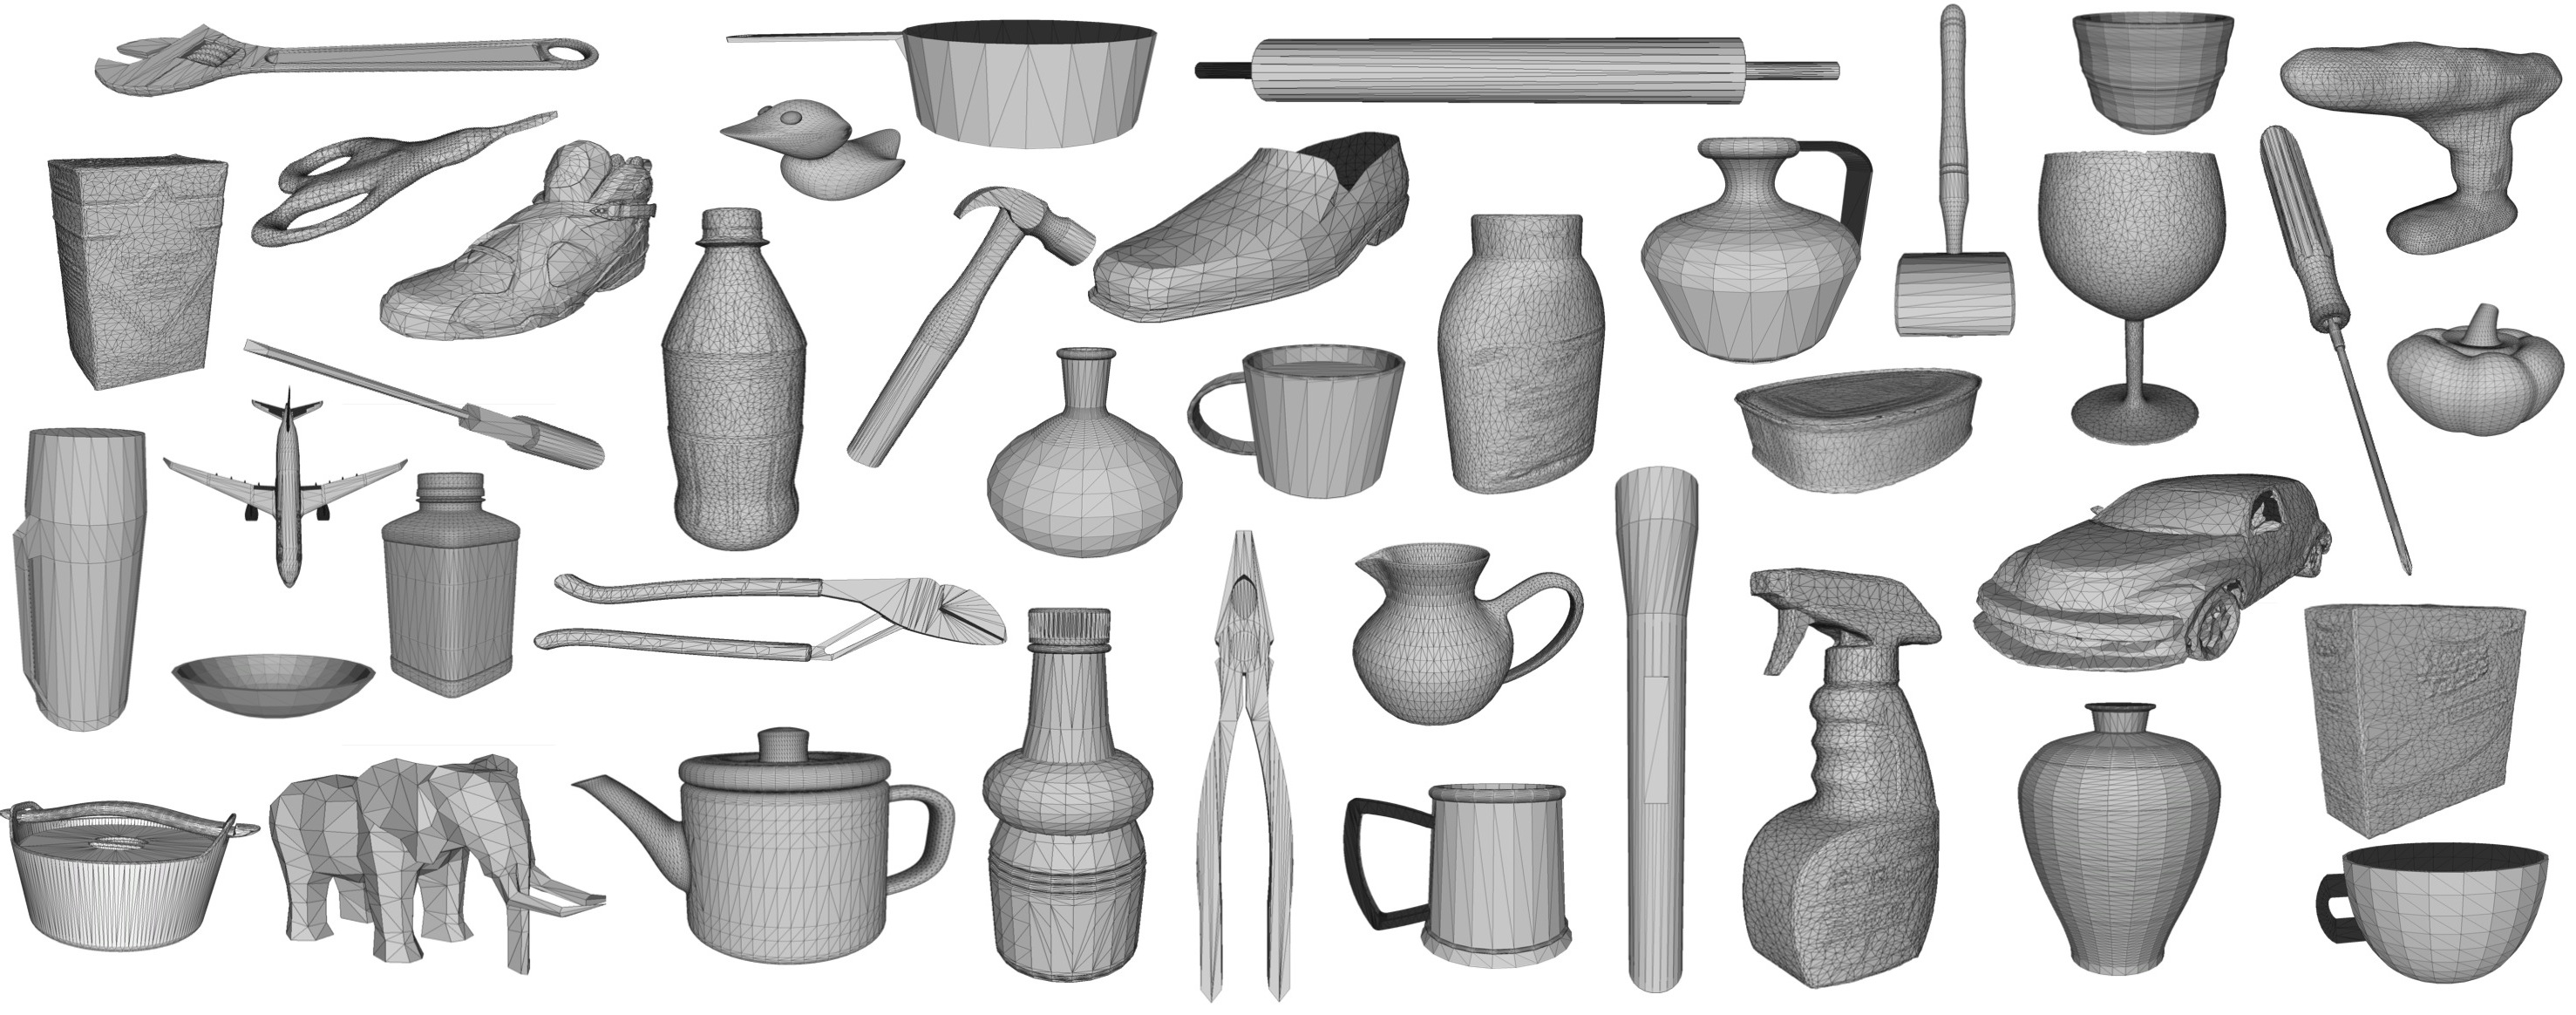
\includegraphics[scale=0.085]{figures/dexnet_collage.jpg}
\caption{Sample of 3D mesh models from the Dex-Net dataset. The dataset currently includes over 10,000 models from laser-scanned datsets such as the KIT object database~\cite{kasper2012kit} and the Yale-CMU-Berkeley object set~\cite{calli2015benchmarking}, and synthetic datasets such as 3DNet\cite{wohlkinger20123dnet}, ModelNet~\cite{wu20143d}, and the SHREC 2014 object retrieval challenge dataset~\cite{li2015comparison}. }
\figlabel{dexnet-teaser}
\vspace*{-15pt}
\end{figure}

Our main contribution is a Multi-Armed Bandit (MAB) algorithm with correlated rewards to scale robust planning by learning from a large dataset of grasps and 3D object models.
Our algorithm is based on Continuous Correlated Beta Processes (CCBPs)~\cite{goetschalckx2011continuous, montesano2012active}, an efficient model for predicting a belief distribution on the quality of each grasp from prior data.

To study scaling effects we develop Dex-Net 1.0, a new dataset of approximately 10,000 3D object models scaled to fit within a PR2 gripper and selected to reflect objects that could be encountered in warehousing or the home such as tooks tableware, boxes, and toys.
~\figref{dexnet-teaser} shows a sample of the objects in the dataset.
Dex-Net contains laser-scanned 3D mesh models from the KIT object database~\cite{kasper2012kit}, the Amazon Picking Challenge objects, BigBIRD~\cite{singh2014bigbird}, and YCB~\cite{calli2015benchmarking} to reflect physical objects commonly used for benchmarking in grasping research.
The dataset also includes synthetic 3D mesh models from shape classification datasets such as 3DNet~\cite{wohlkinger20123dnet}, ModelNet~\cite{wu20143d}, and the SHREC 2014 large scale object retrieval challenge~\cite{li2015comparison} to approach larger scales.
Dex-Net contains approximately 2.5 million parallel-jaw grasps, and each object is labelled with up to 250 grasps and an estimate of the probability of force closure for each under uncertainty in object pose, gripper pose, and friction coefficient.
To the best of our knowledge, this is the largest dataset to-date used for grasping research.
We also incorporate multi-view Convolutional Neural Networks (MV-CNNs)~\cite{su2015multi}, a state-of-the-art method for 3D shape classification, to efficiently retrieve similar 3D objects from Dex-Net for grasp planning at scale. 

We implement our algorithm on Google Compute Engine and store Dex-Net 1.0 on Google Cloud Storage.
Experiments on using our algorithm to plan parallel-jaw grasps with high probability of force closure from 250 candidates suggest that using 10,000 prior object models from Dex-Net can reduce the average number of samples needed to identify a grasp with high quality by $3.5\times$ over a test set of 20 objects.
Experiments on the sensitivity of our algorithm to the similarity metric suggest that measuring false simlarities can lead to a significant decrease in the convergence rate.
\TODO{Update with final results}

 





